\documentclass[german]{beamer}
\usepackage{beamerthemeDarmstadt}
%\usepackage{beamerthemefrankfurt}
%\usepackage{beamerthemecopenhagen}
\usepackage{babel}              % Einstellungen für deutsche Sprache
\usepackage[utf8]{inputenc}
\usepackage[T1]{fontenc}
\usepackage{graphicx}
\usepackage{overpic}
\usepackage{amsmath}
\usepackage{listings} %quelltext-listings
\lstset{basicstyle=\ttfamily\tiny}


\title{Linux Kernel Memory Analysis}
\author{Hagen Fritsch - fritsch+lkma@in.tum.de \\ Dominik Meyer - meyerd@mytum.de}

\date{22.10.2009}

\begin{document}

\frame{\titlepage}

\section{Einführung}
\subsection*{Einführung}
\frame {
\frametitle{Einführung}
 \begin{itemize}
	\item Ziel: Vergleichen zweier Zustände einer VM \\
		$\Rightarrow$ Abstraktion einer High-Level-Repräsentation der Änderungen
	\item Höheres Ziel: Nutzung dieses Ansatzes zur heuristischen Malwareerkennung
	%machine learning approach to detect potentially malicious behaviour
 \end{itemize}
}

\frame{\tableofcontents}

\section{Arbeitsspeicher verstehen}
\subsection{Arbeitsspeicher verstehen}
\frame {
\frametitle{Arbeitsspeicher verstehen}
 \begin{itemize}
 \item Wie versteht der Kernel den Arbeitsspeicher?
  \begin{itemize}
   \item Fest einprogrammiert: Größen von Strukturen, Member-Offsets, Beziehungen
   \item Höhere Abstraktion jedoch vorhanden -> Quelltextebene
   \item Debug-Symbole enthalten die nötigsten Informationen um Strukturen im Arbeitsspeicher zu interpretieren
   \item Globale Variablen sind Einstiegspunkte. Annahme: diese bieten eine gute Abdeckung des Arbeitsspeichers
  \end{itemize}
 \item Die Aufgabe ist zunächst:
   \begin{itemize}
   \item Debug-Symbole verstehen
   \end{itemize}
 \end{itemize}
}

\subsection{Debug-Symbole verstehen}
\begin{frame}[fragile]
\frametitle{Parsing}
  \begin{itemize}
	\item Binärformat aufwendig
	\item Parsen des outputs von \texttt{objdump} mit reg-expressions
	\item Konstruktion entsprechender Type-Objekt-Bäume im Arbeitsspeicher
  \end{itemize}
\begin{lstlisting}[frame=single,caption=A typical objdump structure,label=lst:objdump]
 <1><c6>: Abbrev Number: 4 (DW_TAG_base_type)
    <c7>   DW_AT_byte_size   : 4
    <c8>   DW_AT_encoding    : 5        (signed)
    <c9>   DW_AT_name        : int
 <1><122>: Abbrev Number: 11 (DW_TAG_typedef)
    <123>   DW_AT_name        : (indirect string, offset: 0x82a): __kernel_pid_t
    <127>   DW_AT_decl_file   : 4
    <128>   DW_AT_decl_line   : 14
    <129>   DW_AT_type        : <0xc6>
\end{lstlisting}
\end{frame}

\begin{frame}[fragile]
\frametitle{Verschiedene Typen}
  \begin{itemize}
	\item Jeder Typ wird über eine eigene (teils stub-)Klasse repräsentiert
	\item Alias-Typen wie: typedef, const, member
	\item Standard-Funktionen für jeden Typ wie z.B.:\\
              value(memory\_location)
  \end{itemize}
\begin{lstlisting}[frame=single,caption=Used types,label=lst:types]
structure_type   subroutine_type    variable         formal_parameter*            
union_type       enumeration_typ    const_type       subprogram* 
member           enumerator         typedef          inlined_subroutine*
array_type       pointer_type       base_type        lexical_block*         
subrange_type                                           
\end{lstlisting}
\end{frame}
  
\frame {
\frametitle{Problem der Redundanz}
  \begin{itemize}
    \item Größe und Informationsredundanz: \\
      Binärdump bereits 1GB\\
      benötigt im RAM deutlich mehr Speicher (python-Objekte)
    \item Lösung durch Auflösung von Redundanzen noch während des Parsings
    \begin{itemize}
      \item Vergleichsfunktion für jeden Typ (Name, Größe, Member, rekursiv: basis-Typen, …)
      \item Entfernen von Duplikaten
      \item Noch während des Parsings (RAM), dabei teilweise unvollständige Typen
    \end{itemize}
  \end{itemize}
}

\subsection{Probleme bei der Interpretation}
\frame {
\frametitle{Probleme bei der Interpretation}
 \begin{itemize}
 \item Annahme: Debug-Symbole geben alle nötigen Informationen
 \item Probleme:
  \begin{itemize}
   \item Fehlende Symbole (= fehlende globale Einstiegspunkte)
   \item Unzureichende Informationen über abstraktere Typen wie Strings (allgemein: Arrays ohne Größenangaben)
   \item pointer-magic, type-casts …
  \end{itemize}
 \end{itemize}
}

\frame {
\frametitle{Fehlende Symbole}
 \begin{itemize}
 \item sind während des builds teilweise noch unbekannt
 \item finden sich in der System.map
 \item lesen wir ein
 \end{itemize}
}

\frame {
\frametitle{Fehlende Typinformationen}
 \begin{itemize}
 \item z.B. Größenangaben bei Arrays
 \item oder Pointer, die eigentlich Arrays sind
 \item Lösungsansätze:
  \begin{itemize}
   \item Kopf-in-den-Sand: „ist halt nur ein Element drin“
   \item Heuristic: anhand memory-coverage map (nicht implementiert) % die Größe des Arrays anhand des dortigen unbekannten Speichers bemessen
   \item Manuelle Ansätze: type-casts für bekannte Strukturen (Größe steht in einem anderen Member / Nullterminierte Arrays)

  \end{itemize}
 \end{itemize}
}


\frame {
\frametitle{Wilde Typcasts}
 \begin{itemize}
 \item Linux-Kernel: gute Code-Qualität
 \item aber: viele Hacks
  \begin{itemize}
   \item verkette Listen
   \item Hashtabellen
   \item …
  \end{itemize}
 \end{itemize}
}

\subsubsection{Fallbeispiel: Verkettete Listen}
\begin{frame}[fragile]
\frametitle{Verkettete Listen im Kernel}
  \begin{itemize}
	\item Typlose Standard-Implementierung
        \item Präprocessormakros zum Benutzen notwendig
  \end{itemize}
\begin{lstlisting}[frame=single,caption=Linked lists as used in the linux kernel,label=lst:linkedlists]
//  | next | -->  | next | -->  | first | 
//  | last |  <-- | prev |  <-- | prev  |
struct list_head {
        struct list_head *next, *prev;
};
struct data {
        int attribute;
        struct list_head list;
};
struct data * some_data;
struct data * sample = list_entry(some_data->list.next, struct data, list);
\end{lstlisting}
\end{frame}

\frame {
\frametitle{Verkettete Listen im Kernel: Beispiel \texttt{struct task\_struct}}
 \begin{itemize}
 \item Die \texttt{struct task\_struct} beinhaltet verschiedene Listen
 \item Erster Heuristikansatz: Listen innerhalb von structs zeigen immer auf das selbe Listenmember innerhalb der struct\\
       Hier wäre also angenommen worden: \texttt{task\_struct\_a.children.next} -> \texttt{task\_struct\_b.children}
 \item Leider nur selten korrekt :(
 \end{itemize}
 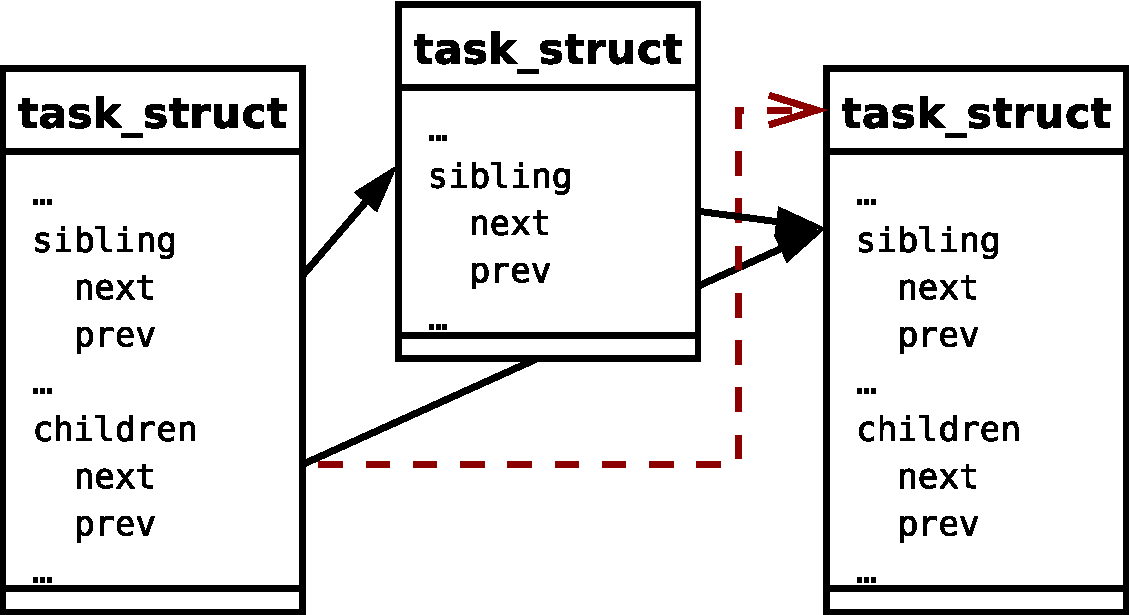
\includegraphics[width=8cm]{../doc/imgs/task_struct_illustration-crop.pdf}
}

\begin{frame}[fragile]
\frametitle{Lösungen für verkettete Listen}
  \begin{itemize}
	\item Kopf-in-den-Sand: „wir verpassen schon nicht so viel“
        \item Manueller Ansatz: Code durchwühlen, Verbindungen herstellen
  \end{itemize}
\begin{lstlisting}[frame=single,caption=Linked lists referencing other types (excerpt from kernel/exit.c),label=lst:linkedliststypes]
void mm_update_next_owner(struct mm_struct *mm)
{
    struct task_struct *c, *p = current;

    list_for_each_entry(c, &p->children, sibling) {
        ...
    }
    ...
}
\end{lstlisting}
  \begin{itemize}
	\item implementiert: Automatisches Durchwühlen des Codes (reg-exp)
        \item hilfreich: lokale Debug-Symbole, minimales Syntax-parsing (wieder reg-exp)
        \item Ergebnis: auto-assoziierte Typen
  \end{itemize}
\end{frame}

\frame {
\frametitle{Zusammenfassung}
 \begin{itemize}
 \item Rekursiver Speicherzugriff über Debug-Symbole
 \item Probleme wie verkettete Listen / Hashtables können überwunden werden \\
       sind aber aufwendig zu implementieren
 \item Wer weiß, was da noch alles im Kernel hockt?
 \item Leider noch keine Statistik über Abdeckung
 \end{itemize}
}

\section{Speicherzugriff}
\subsection{Linear Memory}
\frame {
\frametitle{Speicherzugriff}
\begin{center}
	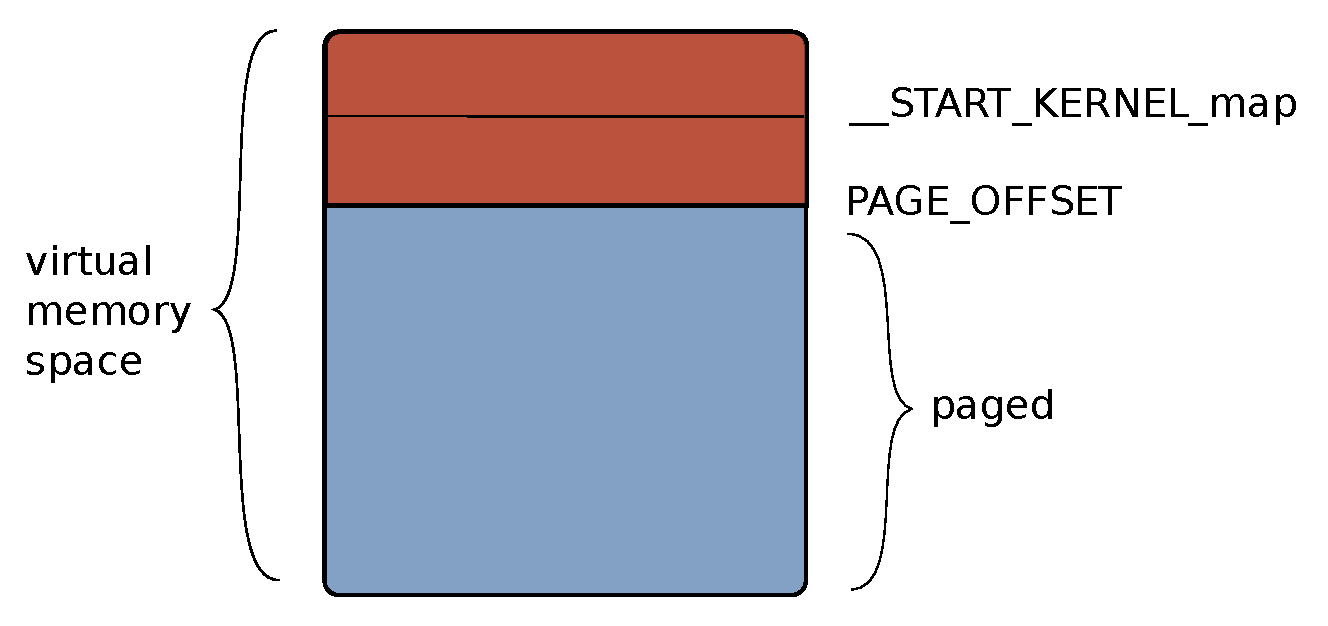
\includegraphics[width=0.8\textwidth]{../doc/imgs/flat_addressing.pdf}
\end{center}

\begin{itemize}
	\item zwei Bereiche
	\item linear: Zugriff durch Subtraktion
	\item paged: Tabellenlookups\\
	\begin{itemize}
		\item allokation im Kernel durch vmalloc()
		\item oder kmalloc()
	\end{itemize}
\end{itemize}

}

\subsection{Paged Memory}
\frame {
\frametitle{Paged Memory}
\begin{center}

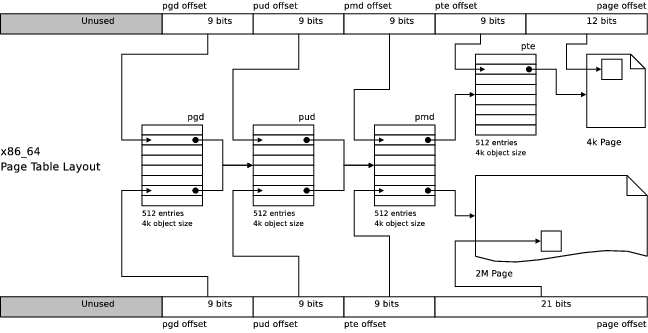
\includegraphics[width=1.0\textwidth]{../doc/imgs/x86_64_pagetable_structure.png}

{{\tiny Source: \url{http://linux-mm.org/PageTableStructure}}}

\end{center}
}

\section{Rootkit Analyse}
\subsection{Generelles Vorgehen}
\frame {
\frametitle{Generelles Vorgehen bei der Analyse}
\begin{itemize}
	\item Snapshots vor/nach Rootkit Installation
	\item Iteration über alle Symbole
	\item Vergleich des Speicherinhalts
	\item bis jetzt: geändert/nicht geändert
\end{itemize}

\begin{itemize}
	\item 3 untersuchte Rootkit Techniken \\
	\begin{itemize}
		\item Syscall Tabelle modifizieren
		\item VFS Einträge erstellen mit bestimmten Eigenschaften
		\item Direkte Manipulation von Kernel Datenstrukturen
	\end{itemize}
\end{itemize}
}

\subsection{Syscall Tabelle}
\frame {
\frametitle{Syscall Tabelle}
\begin{itemize}
	\item Tabelle finden (ab Kernel 2.6) \\
	\begin{itemize}
		\item \texttt{\_text} Section des Kernels im Speicher durchsuchen
		\item \texttt{sidt} Instruction + Interrupt Handler
		\item \texttt{System.map} oder \texttt{/proc/kallsyms}
	\end{itemize}
	\item Schreibzugriff bekommen (ab Kernel 2.6.11)
\end{itemize}
\begin{center}
	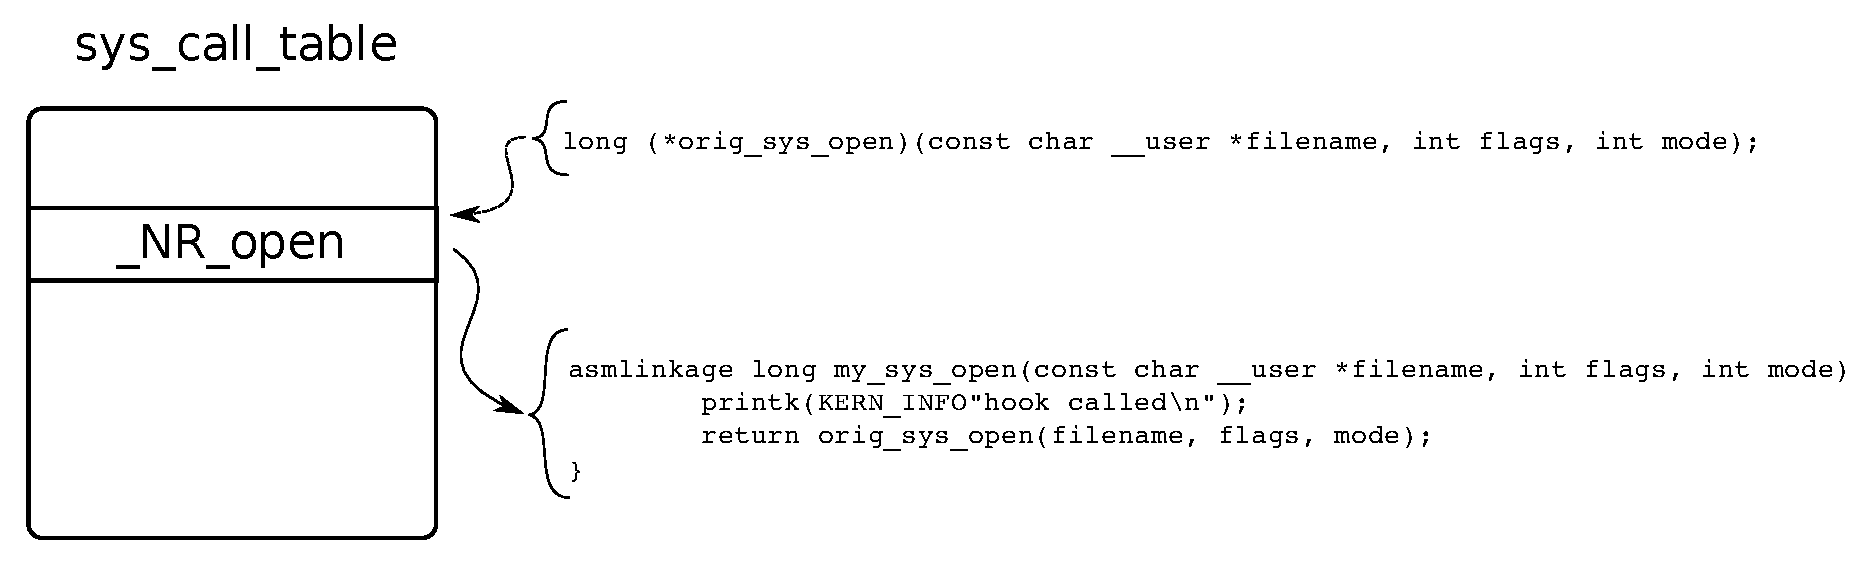
\includegraphics[width=0.95\textwidth]{../doc/imgs/syscall_table_replace.pdf}
\end{center}
}

\subsection{VFS Einträge}
\begin{frame}[fragile]
\frametitle{VFS Einträge}
\begin{itemize}
	\item \texttt{/proc} Dateien erstellen
	\item beim Zugriff \texttt{task\_struct} verfügbar
	\item \texttt{pid, gid, ...} ändern
\end{itemize}
\begin{lstlisting}[frame=single,caption=Proc Eintrag + Rootme,label=lst:procrootkit]
int init_module(void) {
            proc_ent = create_proc_entry(PROCNAME, 0777, NULL);
            ...
            proc_ent->read_proc = rootme;
            ...
}

int rootme(char* buffer, char** buffer_location, off_t offset, int buffer_length, 
       int* eof, void* data) {
            current->uid = 0;
            current->gid = 0;
            current->euid = 0;
            current->egid = 0;
            ...
}
\end{lstlisting}
\end{frame}

\subsection{Direct Kernel Object Manipulation}
\frame {
\frametitle{Direct Kernel Object Manipulation}
\begin{itemize}
	\item Double Linked List aller Module
	\item einfache Pointermanipulation
	\item \texttt{rmmod, lsmod, ...} "`blind"'
\end{itemize}
\begin{center}
	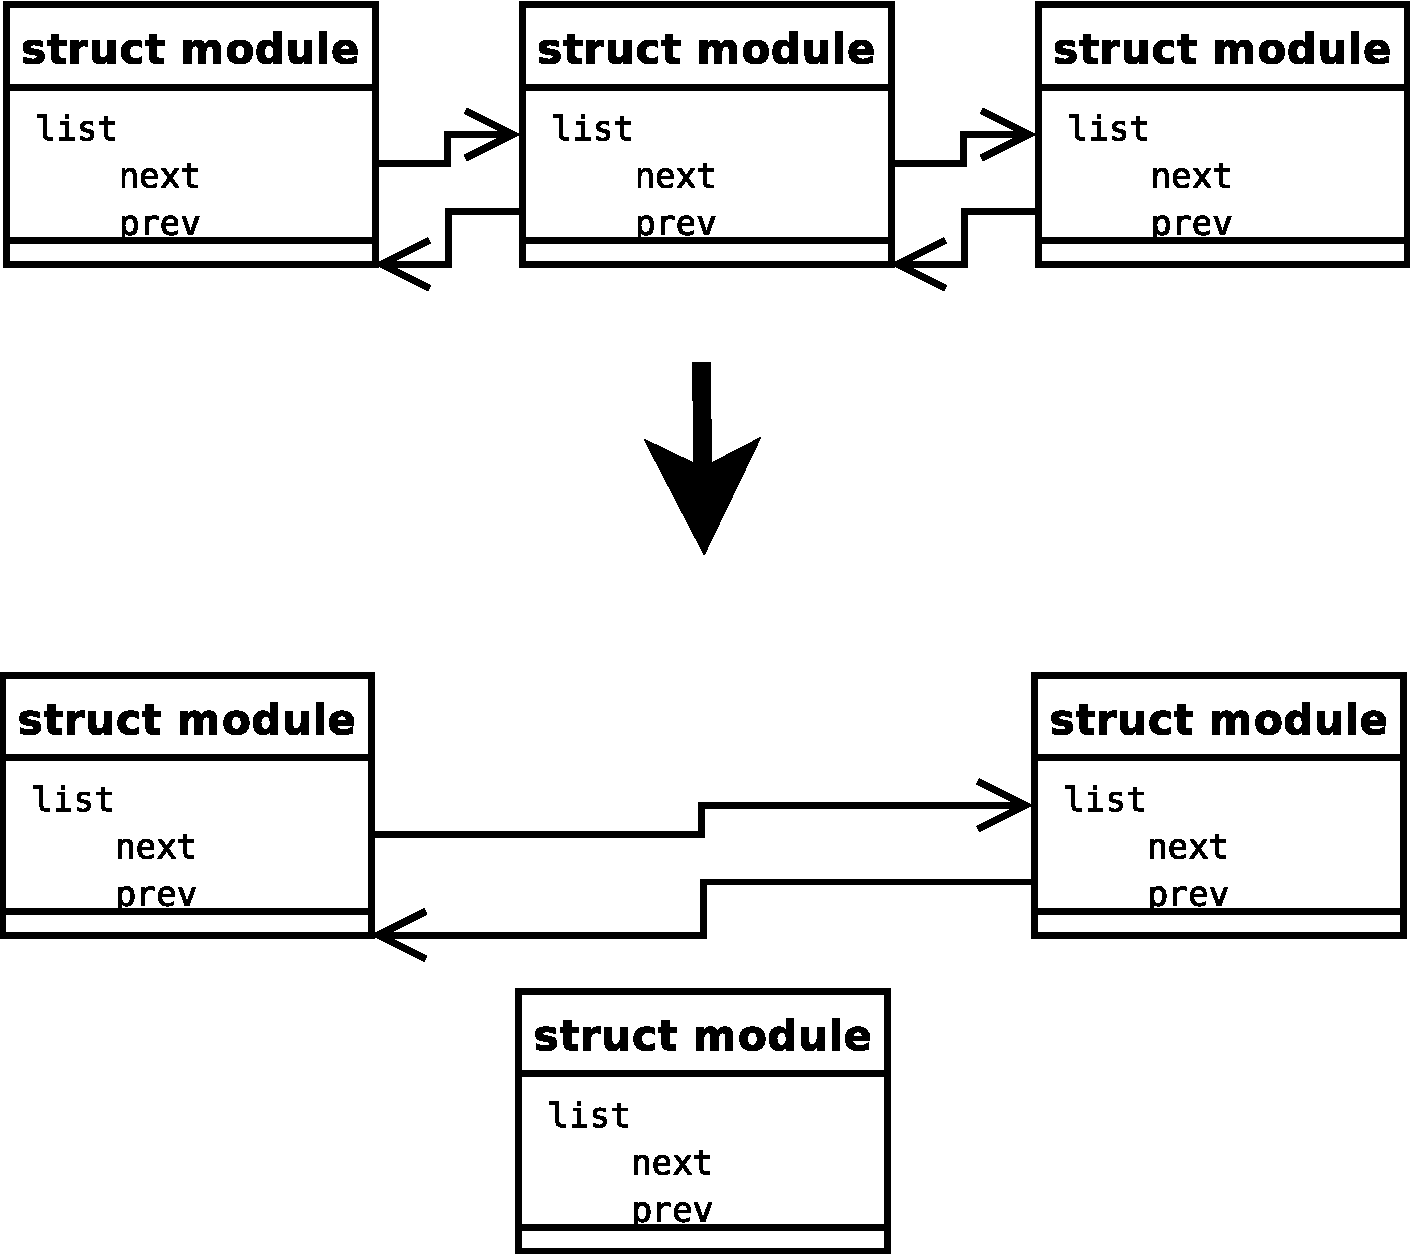
\includegraphics[width=0.45\textwidth]{../doc/imgs/module_list_modification.pdf}
\end{center}
}

\subsection{Herausforderungen}
\frame{
\frametitle{Herausforderungen}
\begin{itemize}
    \item VFS Manipulationen uneindeutig:\\
	\begin{itemize}
		\item \texttt{/proc} Dateien erstellen: unproblematisch
		\item \texttt{uid} ändern ist böse (wirklich?)
	\end{itemize}
    \item System Call Tabelle: \\
    	\begin{itemize}
		\item \texttt{sys\_call\_table} kopieren
		\item Kopie modifizieren
		\item Interrupt Handler/sysenter anpassen
	\end{itemize}
\end{itemize}
}

\frame{
\frametitle{Syscall Interrupt Modifikation}
\begin{center}
	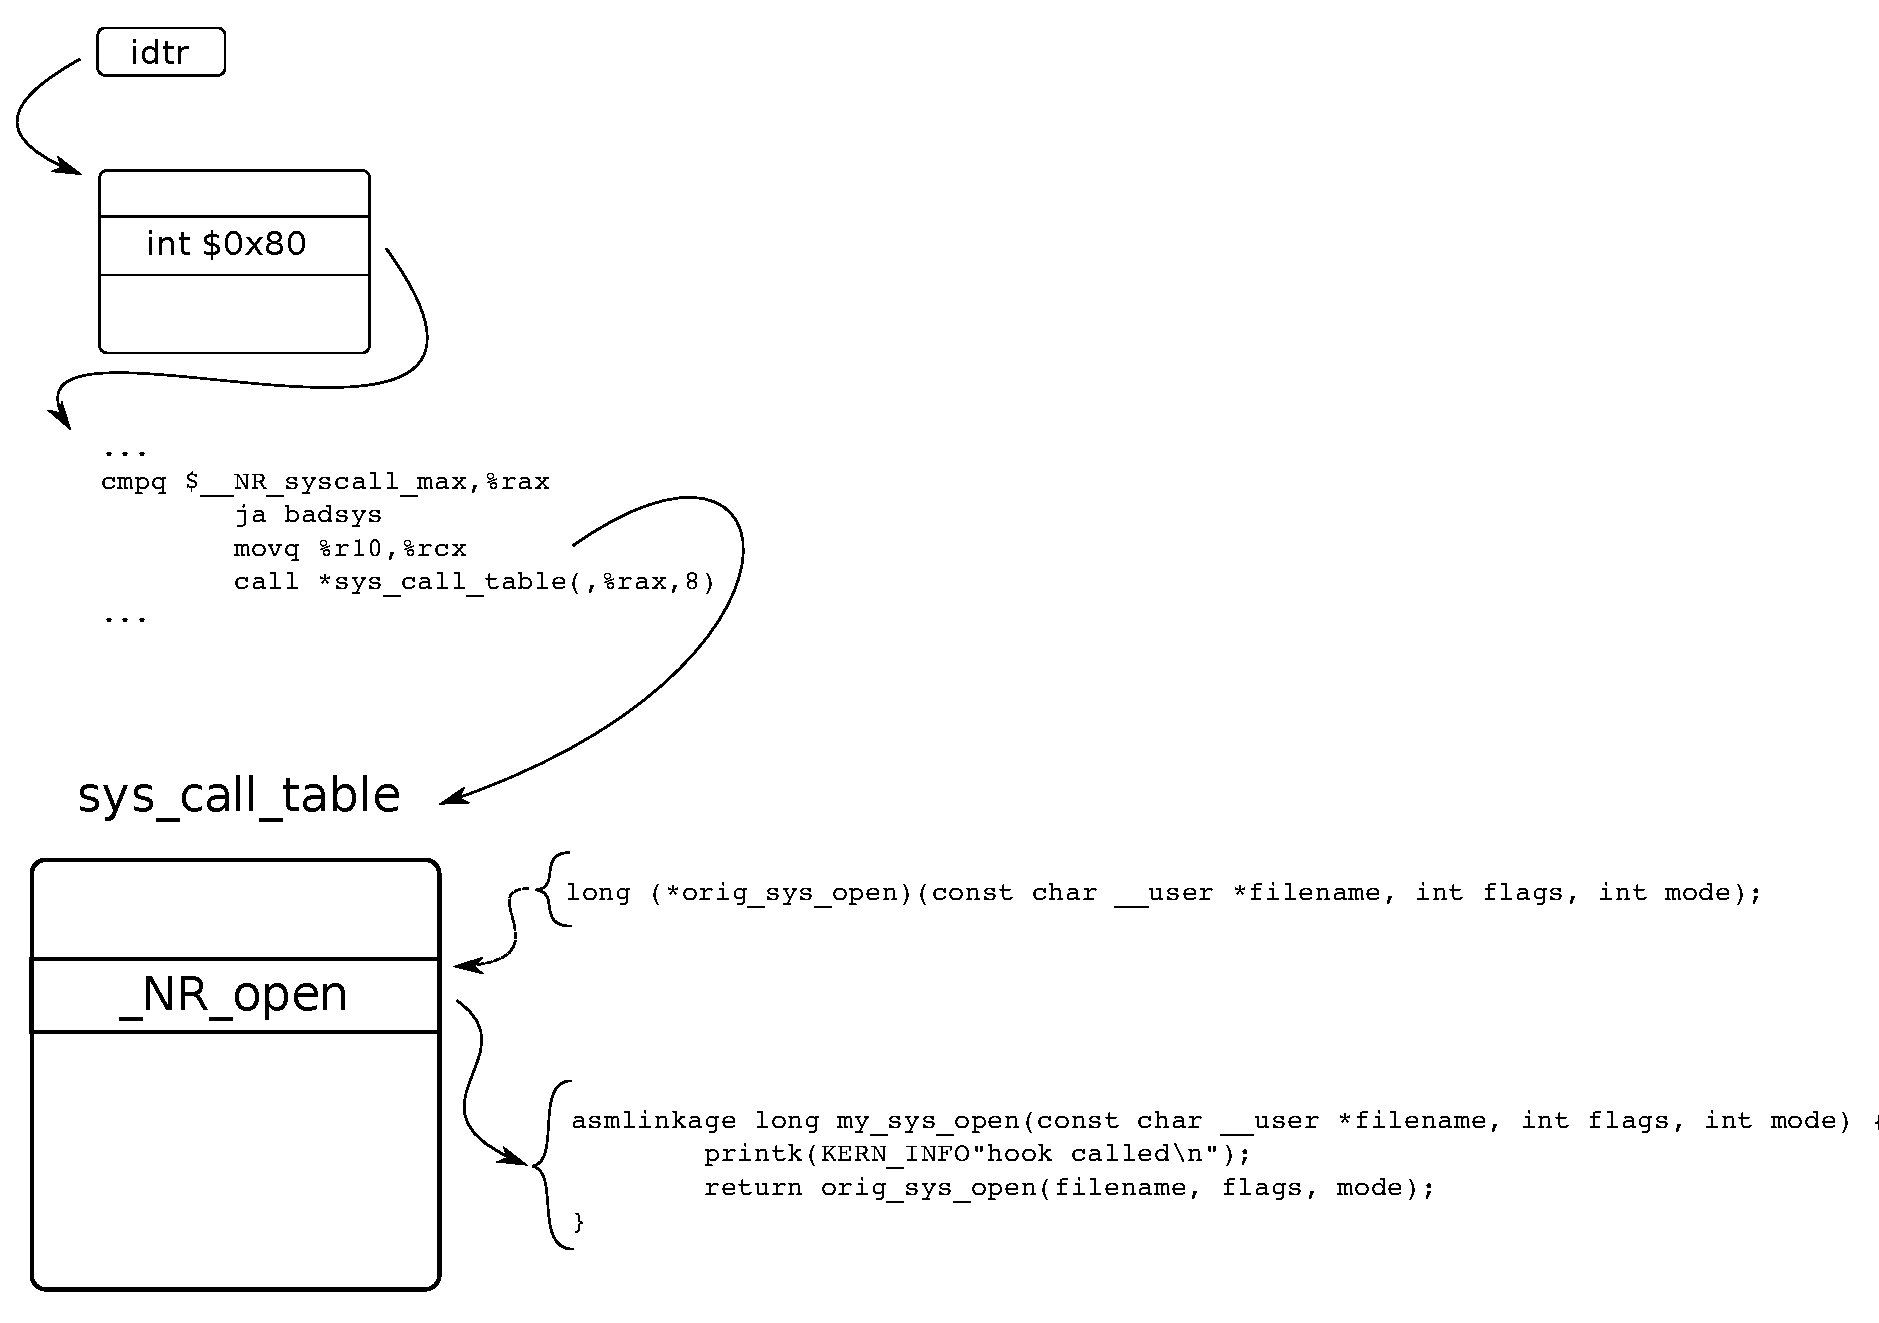
\includegraphics[width=0.8\textwidth]{../doc/imgs/syscall_table_sidt.pdf}

$\Rightarrow$ auch Register überwachen
\end{center}
}

\section{Demo}
\subsection*{Demo}
\frame {
\frametitle{Demo}
\begin{itemize}
	\item Überwachung der \texttt{sys\_call\_table}
	\item Navigation durch die Symbolstruktur
\end{itemize}
}

\frame{
\frametitle{Ende}
\begin{center}
Ende
\end{center}
}

\end{document}
